%%%%%%%%%%%%%%%%%%%%%%%%%%%%%%%%%%%%%%%%%
% Short Sectioned Assignment LaTeX Template Version 1.0 (5/5/12)
% This template has been downloaded from: http://www.LaTeXTemplates.com
% Original author:  Frits Wenneker (http://www.howtotex.com)
% License: CC BY-NC-SA 3.0 (http://creativecommons.org/licenses/by-nc-sa/3.0/)
%%%%%%%%%%%%%%%%%%%%%%%%%%%%%%%%%%%%%%%%%

%----------------------------------------------------------------------------------------
%	PACKAGES AND OTHER DOCUMENT CONFIGURATIONS
%----------------------------------------------------------------------------------------

\documentclass[paper=a4, fontsize=11pt]{scrartcl} % A4 paper and 11pt font size

% ---- Entrada y salida de texto -----

\usepackage[T1]{fontenc} % Use 8-bit encoding that has 256 glyphs
\usepackage[utf8]{inputenc}
%\usepackage{fourier} % Use the Adobe Utopia font for the document - comment this line to return to the LaTeX default

% ---- Idioma --------

\usepackage[spanish, es-tabla]{babel} % Selecciona el español para palabras introducidas automáticamente, p.ej. "septiembre" en la fecha y especifica que se use la palabra Tabla en vez de Cuadro

% NOTA: en caso de problema al compilar, compruebe que tiene el paquete: texlive-babel-spanish.noarch

% ---- Otros paquetes ----

\usepackage{amsmath,amsfonts,amsthm} % Math packages
\usepackage{graphics,graphicx,floatrow} %para incluir imágenes y notas en las imágenes
\usepackage{listings}

\usepackage{url}

%% Define a new 'leo' style for the package that will use a smaller font.
\makeatletter
\def\url@leostyle{%
	\@ifundefined{selectfont}{\def\UrlFont{\sf}}{\def\UrlFont{\small\ttfamily}}}
\makeatother
%% Now actually use the newly defined style.
\urlstyle{leo}
\setlength{\parindent}{12pt}

% Para hacer tablas comlejas
\usepackage{multirow}
\usepackage{threeparttable}

%\usepackage{sectsty} % Allows customizing section commands
%\allsectionsfont{\centering \normalfont\scshape} % Make all sections centered, the default font and small caps

\usepackage{fancyhdr} % Custom headers and footers
\pagestyle{fancyplain} % Makes all pages in the document conform to the custom headers and footers
\fancyhead{} % No page header - if you want one, create it in the same way as the footers below
\fancyfoot[L]{} % Empty left footer
\fancyfoot[C]{} % Empty center footer
\fancyfoot[R]{\thepage} % Page numbering for right footer
\renewcommand{\headrulewidth}{0pt} % Remove header underlines
\renewcommand{\footrulewidth}{0pt} % Remove footer underlines
\setlength{\headheight}{13.6pt} % Customize the height of the header

\numberwithin{equation}{section} % Number equations within sections (i.e. 1.1, 1.2, 2.1, 2.2 instead of 1, 2, 3, 4)
\numberwithin{figure}{section} % Number figures within sections (i.e. 1.1, 1.2, 2.1, 2.2 instead of 1, 2, 3, 4)
\numberwithin{table}{section} % Number tables within sections (i.e. 1.1, 1.2, 2.1, 2.2 instead of 1, 2, 3, 4)

\setlength\parindent{0pt} % Removes all indentation from paragraphs - comment this line for an assignment with lots of text

\newcommand{\horrule}[1]{\rule{\linewidth}{#1}} % Create horizontal rule command with 1 argument of height



\usepackage[utf8]{inputenc}
\usepackage[T1]{fontenc}
\usepackage[spanish]{babel}
\usepackage{times}

\usepackage{color}
\definecolor{gray97}{gray}{.97}
\definecolor{gray75}{gray}{.75}
\definecolor{gray45}{gray}{.45}

\usepackage{listings}
\lstset{ frame=Ltb,
	framerule=0pt,
	aboveskip=0.5cm,
	framextopmargin=3pt,
	framexbottommargin=3pt,
	framexleftmargin=0.4cm,
	framesep=0pt,
	rulesep=.4pt,
	backgroundcolor=\color{gray97},
	rulesepcolor=\color{black},
	%
	stringstyle=\ttfamily,
	showstringspaces = false,
	basicstyle=\small\ttfamily,
	commentstyle=\color{gray45},
	keywordstyle=\bfseries,
	%
	numbers=left,
	numbersep=15pt,
	numberstyle=\tiny,
	numberfirstline = false,
	breaklines=true,
}

% minimizar fragmentado de listados
\lstnewenvironment{listing}[1][]
{\lstset{#1}\pagebreak[0]}{\pagebreak[0]}

\lstdefinestyle{consola}
{basicstyle=\scriptsize\bf\ttfamily,
	backgroundcolor=\color{gray75},
}

\lstdefinestyle{C}
{language=C,
}


\usepackage[pdftex,colorlinks=true,linkcolor=negro,urlcolor=blue]{hyperref,xcolor}
\definecolor{negro}{rgb}{0,0,0}

\graphicspath{ {./images/} }
\usepackage{subfig}
\hypersetup{citecolor=blue}

\title{	
\normalfont \normalsize 
\textsc{{\bf Ingeniería de Servidores (2014-2015)} \\ Grado en Ingeniería Informática \\ Universidad de Granada} \\ [25pt]
\horrule{0.5pt} \\[0.4cm] % Thin top horizontal rule
\huge Memoria Práctica 1 \\ % The assignment title
\horrule{2pt} \\[0.5cm] % Thick bottom horizontal rule
}

\author{Jose Antonio Jiménez Montañés}

\date{\normalsize\today}

%----------------------------------------------------------------------------------------
% DOCUMENTO
%----------------------------------------------------------------------------------------
%
%\begin{figure}[H]
%	\centering
%	\includegraphics[width=0.5\textwidth]{gull}
%	\caption{Texto Prueba}
%	\label{fig:ddd}
%\end{figure}


%\cite{p1}

\begin{document}

\maketitle % Muestra el Título

\newpage %inserta un salto de página

\tableofcontents % para generar el índice de contenidos

\listoffigures

%\listoftables 

\newpage

%----------------------------------------------------------------------------------------
%	Cuestion 1
%----------------------------------------------------------------------------------------
\section{¿Qué modos \cite{01p11} y tipos \cite{02p12} \cite{02p13} de “virtualización” existen?}
\LARGE {\textbf{Modos}} 
\\
\normalsize
	\textbf{HVM} (Hardware virtualizado): Es una virtualización en el que el sistema BIOS del servidor carga una imagen del sistema  desde la que crea la máquina virtual. En algunas fuentes también se le llama virtualización completa.
\\
\\
	\textbf{PVHVM} (Hardware virtualizado con los controladores para-virtualizados): Es igual a HVM excepto que los controladores son paravirtualizados para mejorar el rendimiento de la máquina virtual. En algunas fuentes también se le llama virtualización parcial.
\\
\\
	\textbf{PVM} (Paravirtualizado): Es una manera de virtualizar un sistema que llamaremos cliente en otro que llamaremos anfitrión. En algunas fuentes se le denomina virtualización por S.O.
\\
\\
	\textbf{OVM/SPARC} (Oracle VM Server para SPARC): Es un modo especial de Oracle para servidores e hipervisores que utilizan Oracle VM Server para SPARC.
\\
\\
\LARGE {\textbf{Tipos}} 
\\
\normalsize
	\textbf{Plataformas(o de servidores):} Consiste en separar un sistema operativo de los recursos de la plataforma anfitrión. De esta forma se pueden ejecutar varios sistemas operativos de cualquier plataforma al misma tiempo en una misma máquina.
\\
	\textbf{Recursos:} Consiste en virtualizar recursos específicos del sistema como pueden ser:
\\
		• Redes: Reproducción completa en software de una red física. Es altamente escalable y proporciona niveles altos de agilidad y eficiencia.
\\
		• Escritorios: Proporciona soluciones para ofrecer acceso a escritorios remotos, ideales para empleados externos (otros países etc.), teletrabajo, etc.
\\
		• Aplicaciones: La virtualización es a nivel de aplicación y es ideal para el mundo empresarial (ERP, CRM, bases de datos… etc.). Proporciona más seguridad y alta disponibilidad.
\\
		• Almacenamiento: Mejora el aprovechamiento y eficacia de los sistemas de almacenamiento así como una mejor gestión de estos recursos.
\clearpage
%------------------------------------------------
% CUESTION 2
%------------------------------------------------
\section{Muestre los precios y características de varios proveedores de VPS (Virtual Private Server) y compare con el precio de servidores dedicados (administrados y no administrados).\cite{03p21} \cite{03p22} \cite{03p23} \cite{03p24}}

\begin{figure}[H]
	\centering
	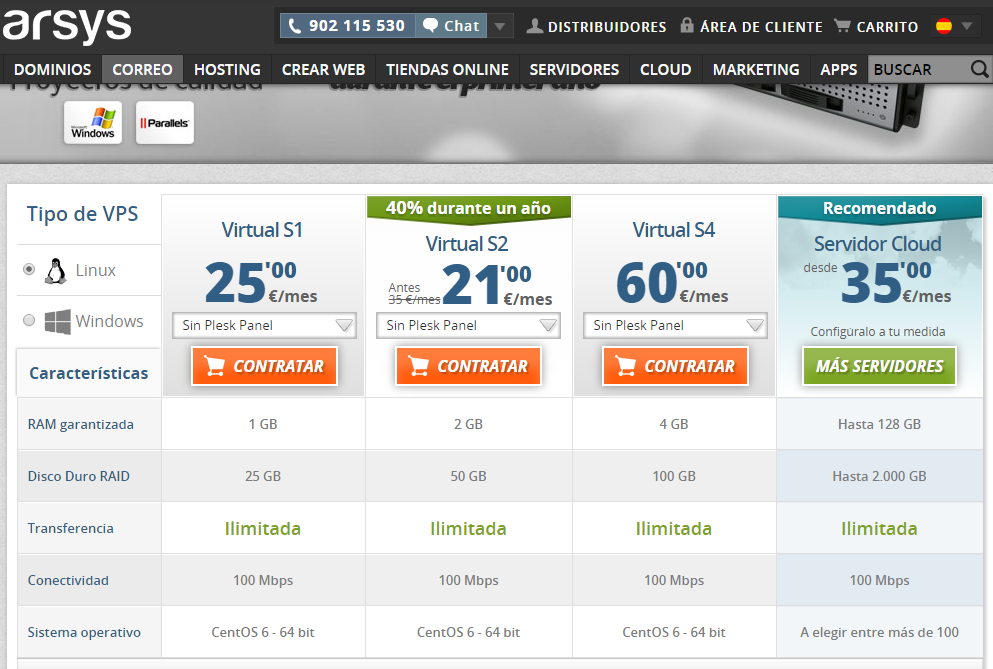
\includegraphics[width=0.7\textwidth]{images/2/arsys}
	\caption{Precios de VPS en Arsys}
	\label{fig:c0201}
\end{figure}


\begin{figure}[H]
	\centering
	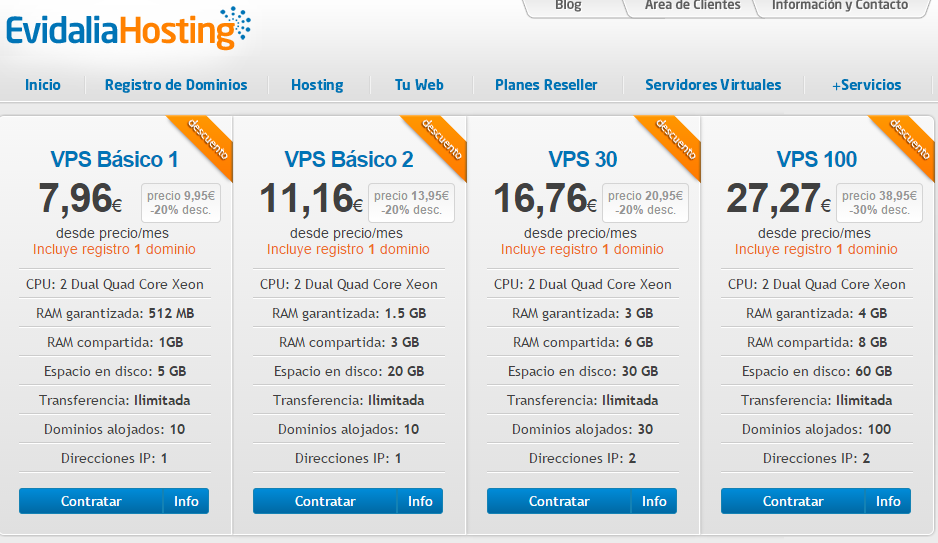
\includegraphics[width=0.7\textwidth]{images/2/evidalia}
	\caption{Precios de VPS en Evidalia}
	\label{fig:c0202}
\end{figure}


\begin{figure}[H]
	\centering
	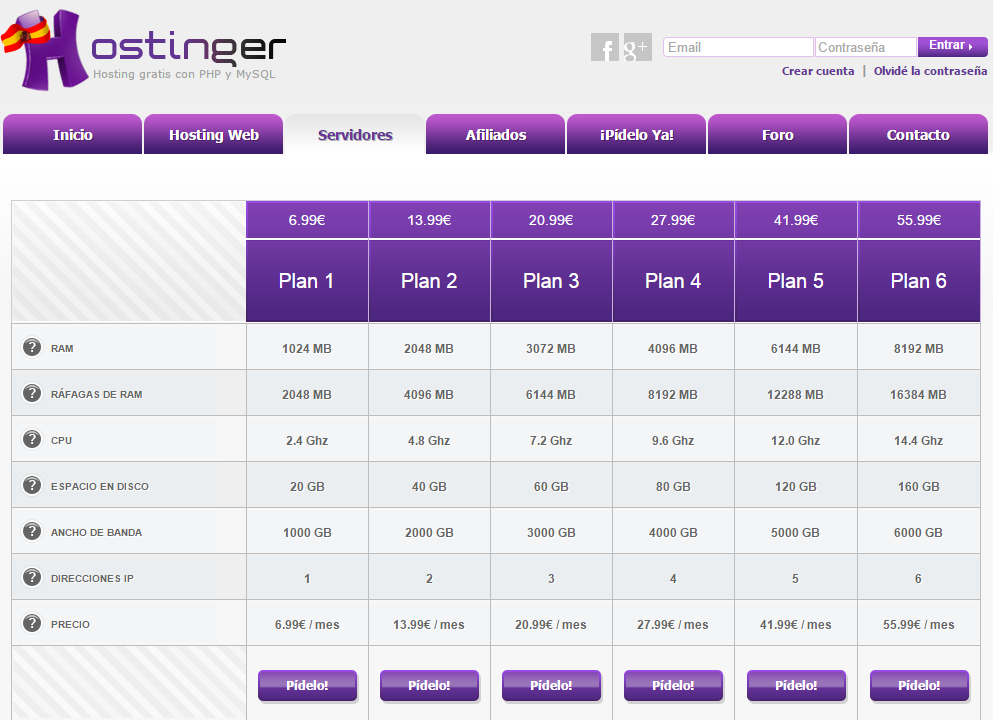
\includegraphics[width=0.7\textwidth]{images/2/hostinger}
	\caption{Precios de VPS en Hostinger}
	\label{fig:c0203}
\end{figure}


\begin{figure}[H]
	\centering
	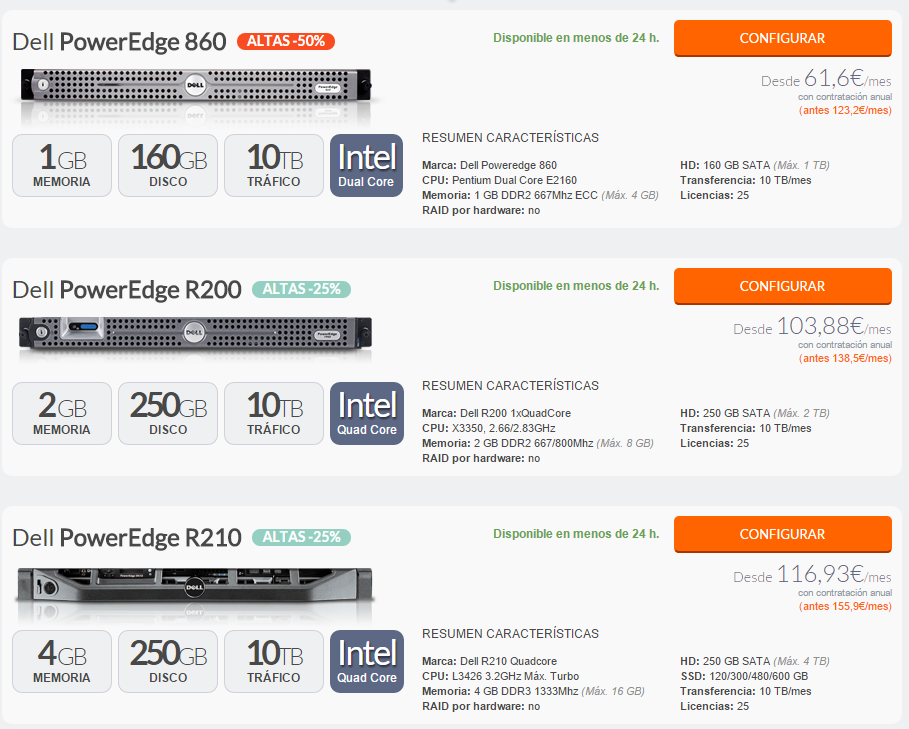
\includegraphics[width=0.7\textwidth]{images/2/dedidado_admin_dinahosting}
	\caption{Precios de servidores dedicados con administración en Dinahosting}
	\label{fig:c0204}
\end{figure}

\begin{figure}[H]
	\centering
	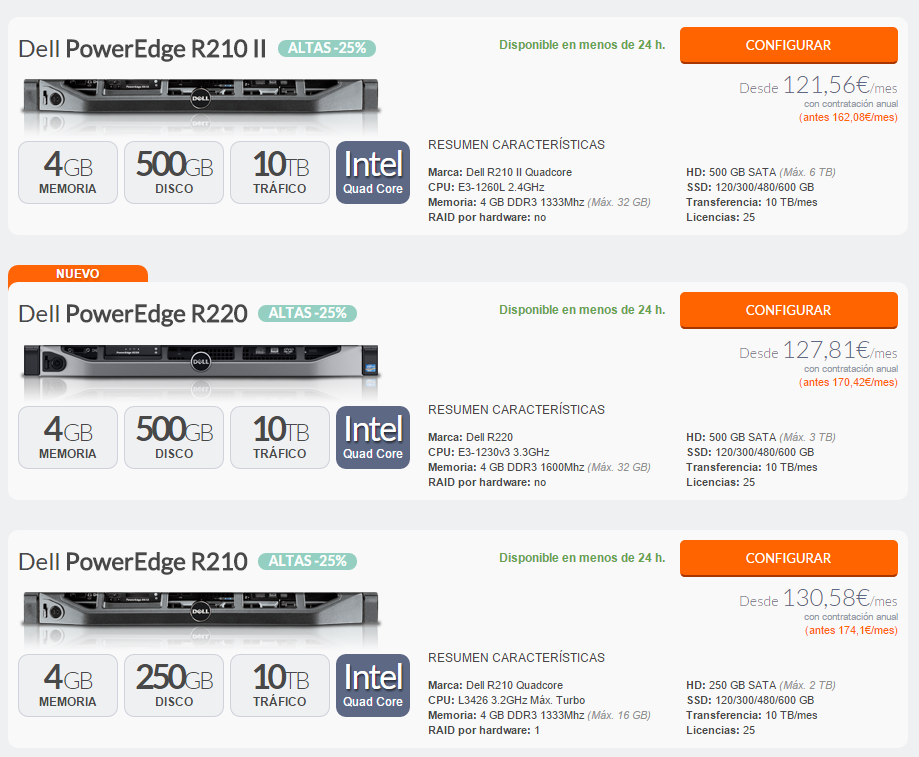
\includegraphics[width=0.7\textwidth]{images/2/dedidado_admin_dinahosting2}
	\caption{Precios de servidores dedicados con administración en Dinahosting}
	\label{fig:c0205}
\end{figure}

\begin{figure}[H]
	\centering
	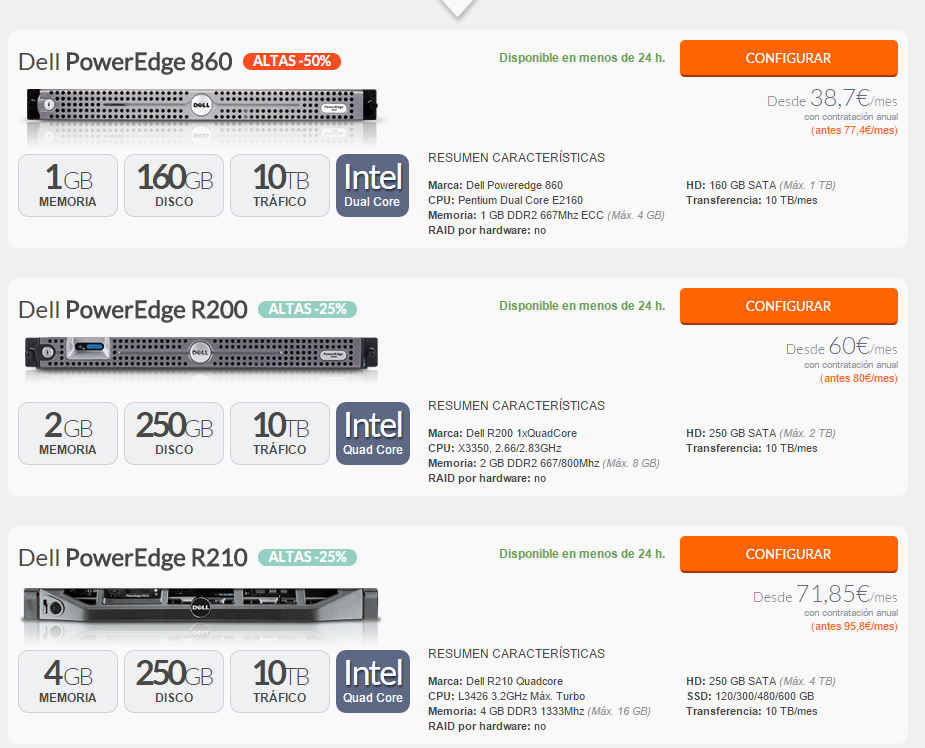
\includegraphics[width=0.7\textwidth]{images/2/dedidado_NOadmin_dinahosting}
	\caption{Precios de servidores dedicados sin administración en Dinahosting}
	\label{fig:c0206}
\end{figure}

\begin{figure}[H]
	\centering
	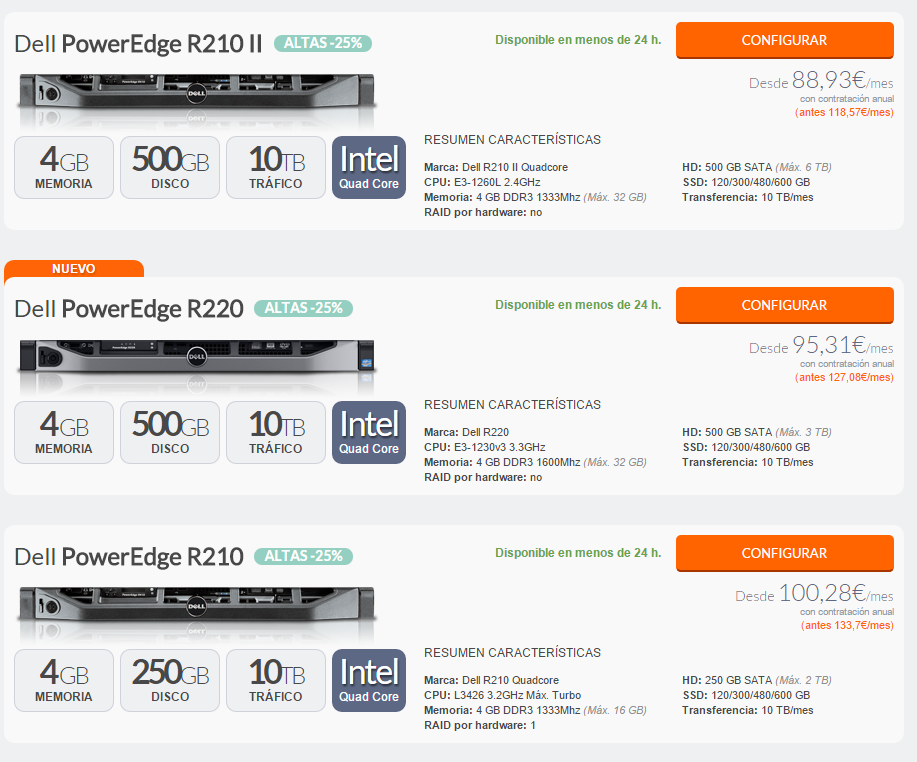
\includegraphics[width=0.7\textwidth]{images/2/dedidado_NOadmin_dinahosting2}
	\caption{Precios de servidores dedicados sin administración en Dinahosting}
	\label{fig:c0207}
\end{figure}


Podemos concluir que los servidores virtuales ofrecen una mayor ventaja respecto al precio, posteriormente los dedicados no administrados y finalmente los más caros serian los dedicados administrados.\\
\clearpage
%----------------------------------------------------------------------
% CUESTION 3	
%----------------------------------------------------------------------------------------

\section{¿Qué otros software de virtualización existen además de VMWare y Virtual Box? \cite{04p31}}

\textbf{Citrix}
\\
• XenServer\\
\\
\textbf{Microsoft}\\
• Microsoft Virtual PC\\
• Windows Server 2008 R2 Hyper-V\\
• Microsoft Enterprise Desktop Virtualization (MED-V)\\
\\
\textbf{Red Hat}\\
• KVM y SPICE\\
\\
\textbf{Virtual Bridges}\\
• VERDE\\
\\
\textbf{Proxmox}\\
• OpenVZ \\
\\
\textbf{Parallels}\\
• Parallels Desktop\\
\\
\textbf{Otros}
• Virtual Iron\\
• Adeos\\
• Mac-on-Linux\\
\\

%-------------------------------------------------------------------------------------------
% CUESTION 4
%--------------------------------------------------------------------------------------------
\section{Enumere algunas de las innovaciones en Windows 2012 R2 respecto a 2008R2 \cite{05p41}}

-Ahora con 2012 se pueden administrar los dispositivos móviles directamente a través del panel de instrumentos.\\
-Se mejora el sistema de restauración de los clientes, soportando restauración por Red en vez de imágenes DVD.\\
-Se mejora el acceso web Remoto siendo compatible con HTML5 y dispositivos táctiles.\\
-Integración del sistema con los servicios de Nube incluyendo Microsoft Azure Active Directory.\\
-Soporta volúmenes multiterabyte.\\
-Replica HyperV: replica todos los cambios de una máquina virtual a una máquina virtual homóloga hospedada por un servidor diferente.\\
\clearpage
%----------------------------------------------------------------------------------------
% CUESTION 5
%----------------------------------------------------------------------------------------
\section{¿Que empresa hay detrás de Ubuntu? ¿Qué otros productos/servicios ofrece? ¿Que es MAAS (https://maas.ubuntu.com/)? \cite{06p51} \cite{06p52}}

a) La empresa que hay detrás de Ubuntu es Canonical.\\\\
b) Productos y Servicios.\\
-Paisaje: Herramienta para crear, administrar y escalar los sistemas Cloud.\\
-Juju y MAAS: Herramientas para usar sistemas Cloud propios.\\
-Ubuntu Advantage: Es un paquete de apoyo profesional de expertos de Canonical para realizar desplieges de Ubuntu con soporte 24/7 y acceso Landscape.\\\\
c) MAAS\\
-Es un proyecto de canonical en el cual se facilita la instalación y despliegue de computación en la nube escalable. Este proyecto permite tratar los servidores físicos como máquinas virtuales en la nube.\\

%----------------------------------------------------------------------------------------
% CUESTION 6
%----------------------------------------------------------------------------------------
\section{¿Que relación tiene esta distribución con Red Hat y con el proyecto Fedora? \cite{07p61}}
Tanto Red Hat con “Red Hat Entreprise Linux” como Fedora con “Fedora Linux” son tecnologías de código abierto. Fedora es construido por la comunidad en su beneficio y Red Hat Entreprise Linux es utilizado como plataforma de TI para empresas.\\
Ambos organismos se benefician mutuamente. Fedora desde el patrocinio y la retroalimentación de Red Hat, y Red Hat consiguiendo innovación de vanguardia de la comunidad en general que le permite madurar rápidamente su tecnología.\\
\clearpage
%----------------------------------------------------------------------------------------
% CUESTION 7
%----------------------------------------------------------------------------------------

\section{Indique que otros SO se utilizan y el porcentaje de uso (no olvide poner la fuente de donde saca la información y preste atención a la fecha de esta) \cite{08p71}}

La mayoría del mercado lo abarca Microsoft sobre todo con Windows 7 que acapara casi la mitad del mercado, lejos están sistemas como MacOS o Linux.\\
\begin{figure}[H]
	\centering
	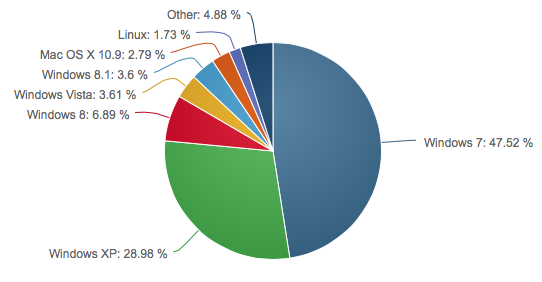
\includegraphics[width=1\textwidth]{images/7}
	\caption{Uso de otros sistemas operativos en 2014}
	\label{fig:c0701}
\end{figure}

%----------------------------------------------------------------------------------------
% CUESTION 8
%----------------------------------------------------------------------------------------
\section{a)¿De que es el acrónimo RAID? b)¿Que tipos de RAID hay? c)¿Que diferencia hay entre RAID mediante SW y mediante HW? \cite{09p81}}
		 
a) Redundant Array of Independent Disks\\\\
b) Hay 3 tipos:\\
Puros: (0, 1, 2, 3, 4, 5, 5E, 6, 6E).\\
Anidados o Híbridos: (0+1, 10, 30, 50, 60, 100, 101).\\
Propietarios: (1.5, 50EE, 7, S, Z, SERVER RAID).\\\\
c) Por HW, el subsistema presenta un único disco a la maquina por conjunto de discos RAID. Permite “Hot-swapping” y es más rápido que por SW.\\
Por SW implementa los niveles RAID en el código del núcleo. Es el método más barato y su rendimiento es mayor.
\clearpage
%----------------------------------------------------------------------------------------
% CUESTION 9
%----------------------------------------------------------------------------------------
\section{a)Que es LVM?,b)¿Que ventaja tiene para un servidor de gama baja? c)Si va a tener un servidor web, ¿le daria un tamano grande o pequeno a /var? \cite{10p91}}

a) Es un Administrador de volúmenes lógicos para Linux\\\\
b) Ayuda a administrar el sistema de particionado de forma eficiente, agregando o eliminando espacio particionado en carpetas.\\\\
c) Grande ya que es el directorio donde se almacena los directorios y ficheros de bloqueo, datos de administración y registro además de los ficheros temporales.\\
Así mismo en /var/lib están las bases de datos del sistema y en /var/spool se encuentran diversos subdirectorios de subsistemas que almacenan ficheros de datos.

%----------------------------------------------------------------------------------------
% CUESTION 10
%----------------------------------------------------------------------------------------
\section{¿Debemos cifrar también el volumen que contiene el espacio para swap? ¿y el volumen en el que montaremos /boot?}

a) Si, para proteger nuestros procesos poco activos de que otros les cierren (hackers, virus, etc).\\\\
b) No, ya que está dedicado a guardar el arranque del sistema, si se cifra el sistema no podría arrancar.
\clearpage
%----------------------------------------------------------------------------------------
% CUESTION 11
%----------------------------------------------------------------------------------------
\section{¿Que otro tipo de usos de una partición le permite configurar el asistente de instalación?. ¿Cual es la principal diferencia entre ext4 y ext2? \cite{11p111}}

a)\begin{figure}[H]
	\centering
	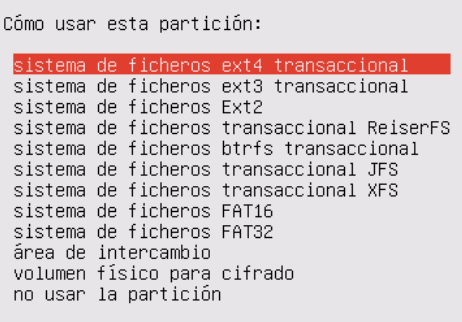
\includegraphics[width=1\textwidth]{images/11}
	\caption{Captura de los tipos de sistema de ficheros que admite Ubuntu Server 14.04}
	\label{fig:c1101}
\end{figure}


b) La principal diferencia es que ext2 no implementa el registro de diario. Además ext4 soporta volúmenes de gran tamaño (1Exabyte) y fichero de hasta 16TB, mientras que ext2 solo soporta 2TB de tamaño de fichero.
\clearpage
%----------------------------------------------------------------------------------------
% CUESTION 12
%----------------------------------------------------------------------------------------
\section{Muestre como ha quedado el disco particionado una vez el sistema está instalado}

Con la orden ‘df –h’ podemos ver como ha quedado:\\
\begin{figure}[H]
	\centering
	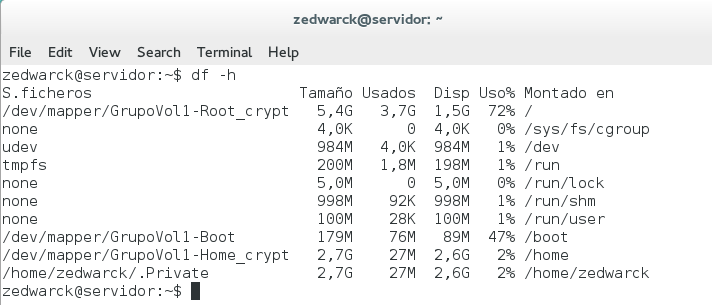
\includegraphics[width=1\textwidth]{images/12}
	\caption{Captura del disco particionado después de configurar RAID1}
	\label{fig:c1201}
\end{figure}

%----------------------------------------------------------------------------------------
%CUESTION 13
%----------------------------------------------------------------------------------------
\section{a)¿Como ha hecho el disco 2 “arrancable”?,b)¿Que hace el comando grub-install? c)¿Que hace el comando dd?}

a) Haciendo un ‘grub-install sdb’ además de tener la flag de active en on (esto se hace en el sistema de particionado en la instalación).\\\\
b) Instala el gestor de arranque Grub en el disco indicado.\\\\
c) Realiza copias de ficheros de un determinado formato especificado en la misma línea de comandos.
\clearpage
%----------------------------------------------------------------------------------------
% CUESTION OPCIONAL 1
%----------------------------------------------------------------------------------------
\section{Cuestión Opcional 1: Muestre (con capturas de pantalla) como ha comprobado que el RAID1 funciona}

Consultando el archivo /proc/mdstat. Si los 2 discos RAID están funcionando correctamente el sistema raid se marcará con una doble U (‘UU’) si alguno fallase mostraría solo una U con una barra baja en el lugar del disco con fallo (‘\_U’).\\
\begin{figure}[H]
	\centering
	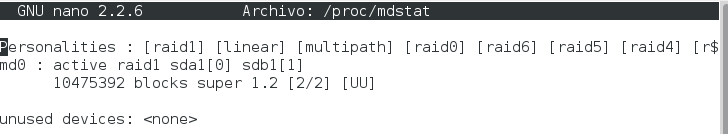
\includegraphics[width=1\textwidth]{images/op1}
	\caption{Comprobación del estado del RAID1}
	\label{fig:co101}
\end{figure}
%----------------------------------------------------------------------------------------
% CUESTION 14
%----------------------------------------------------------------------------------------
\section{¿Que diferencia hay entre Standard y Datacenter? \cite{12p141}}

Según Microsoft:\\\\
"Tanto la edición Standard como la edición Datacenter proporcionan el mismo conjunto de características, lo único que diferencia las ediciones es el número de Máquinas Virtuales (VMs). Una licencia de edición Standard le da derecho a ejecutar hasta dos VMs en hasta dos procesadores (sujeto a los derechos de uso de VM descritos en el documento de Derechos de uso de producto). Una licencia de edición Datacenter le da derecho a ejecutar un número ilimitado de VMs en hasta dos procesadores."\\

%----------------------------------------------------------------------------------------
% CUESTION 15
%----------------------------------------------------------------------------------------
\section{Continue usted con el proceso de definición de RAID1 para los dos discos de 50MiB que ha creado. Muestre el proceso con capturas de pantalla.}
\begin{figure}[H]
	\centering
	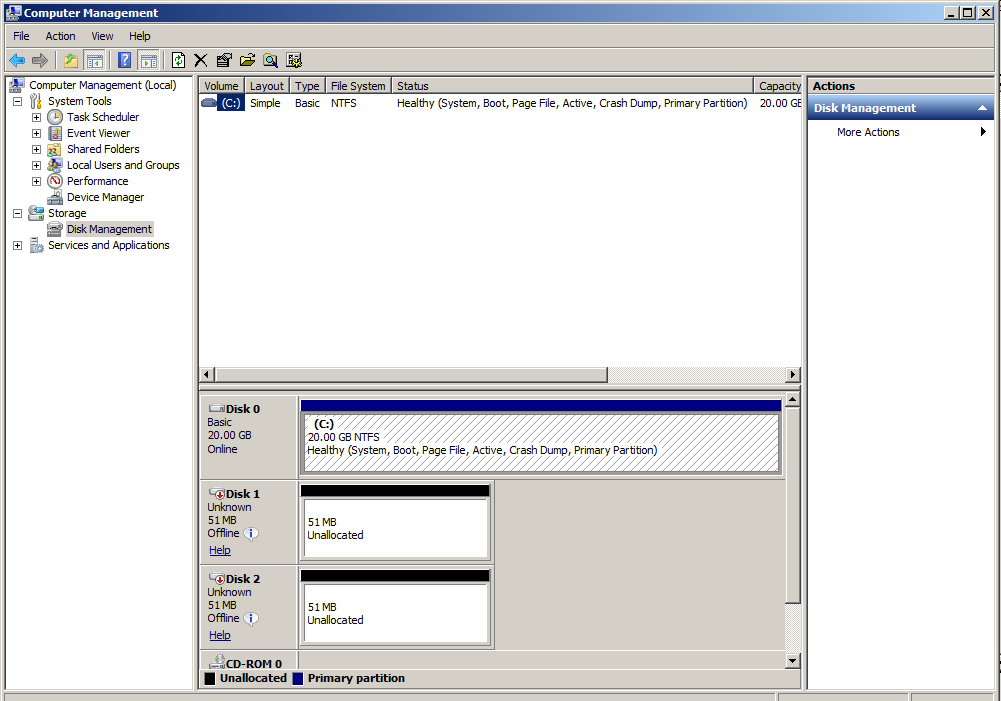
\includegraphics[width=0.8\textwidth]{images/15/1}
	\caption{Visualización del sistema de partición antes de preparar el RAID1}
	\label{fig:c1501}
\end{figure}
\begin{figure}[H]
	\centering
	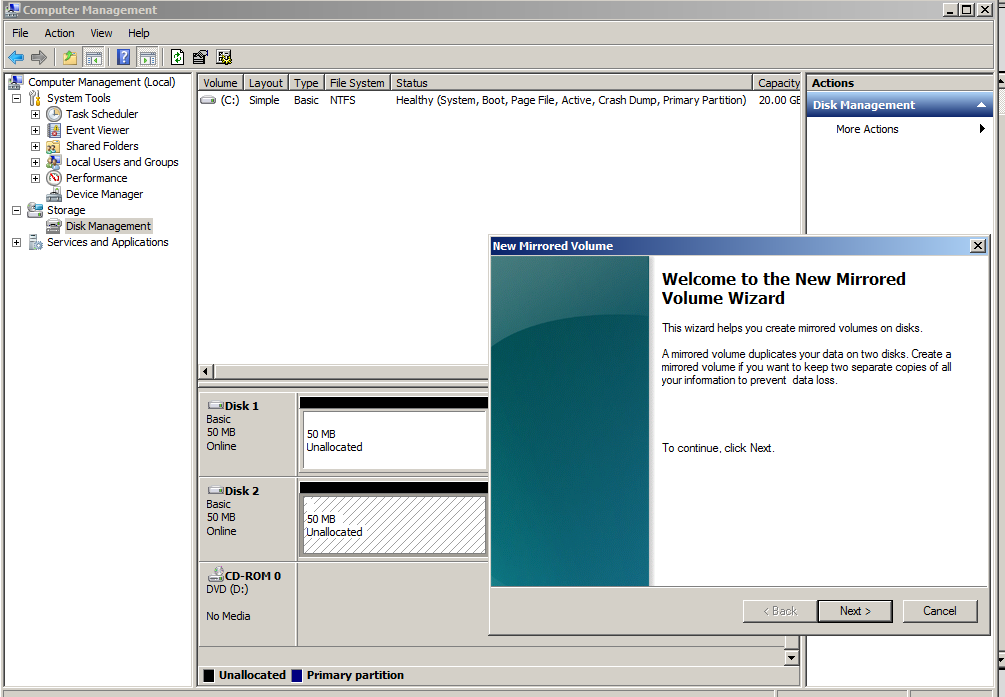
\includegraphics[width=0.8\textwidth]{images/15/2}
	\caption{Inicio de la configuración del RAID1}
	\label{fig:c1502}
\end{figure}
\begin{figure}[H]
	\centering
	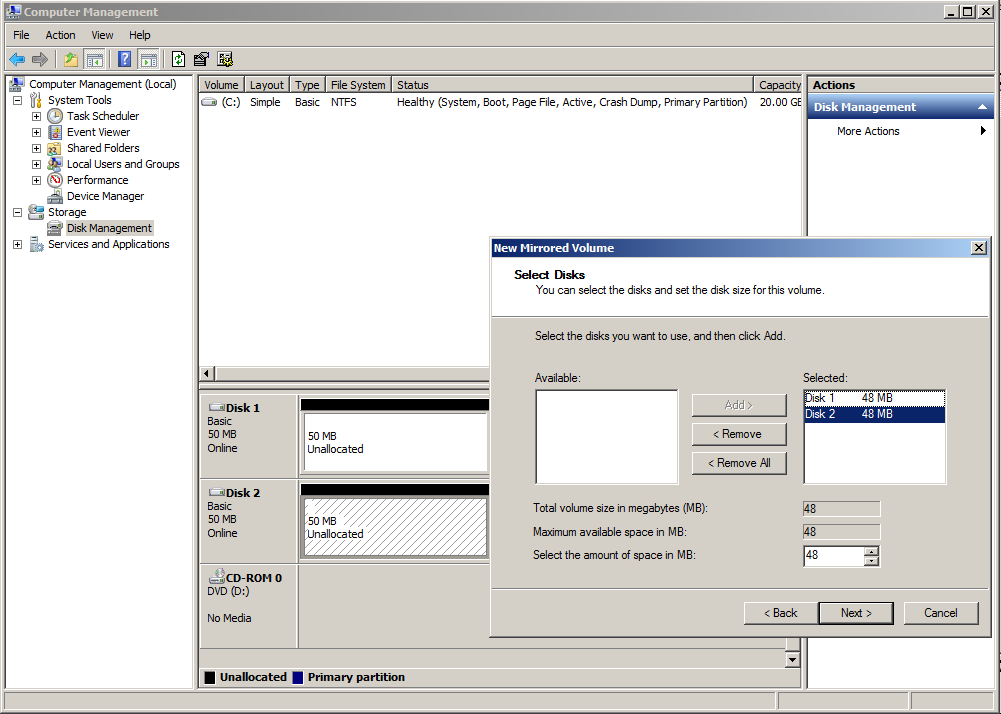
\includegraphics[width=0.8\textwidth]{images/15/3}
	\caption{Elección de los discos RAID1}
	\label{fig:c1503}
\end{figure}
\begin{figure}[H]
	\centering
	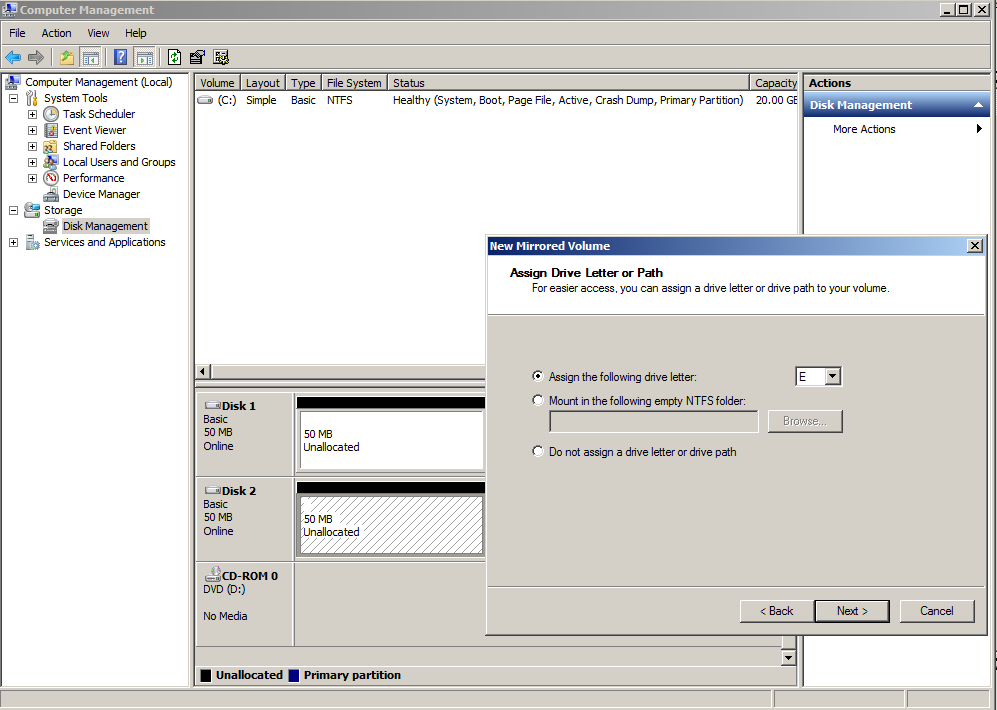
\includegraphics[width=0.8\textwidth]{images/15/4}
	\caption{Asignación del montaje para el RAID1 (letra o carpeta)}
	\label{fig:c1504}
\end{figure}
\begin{figure}[H]
	\centering
	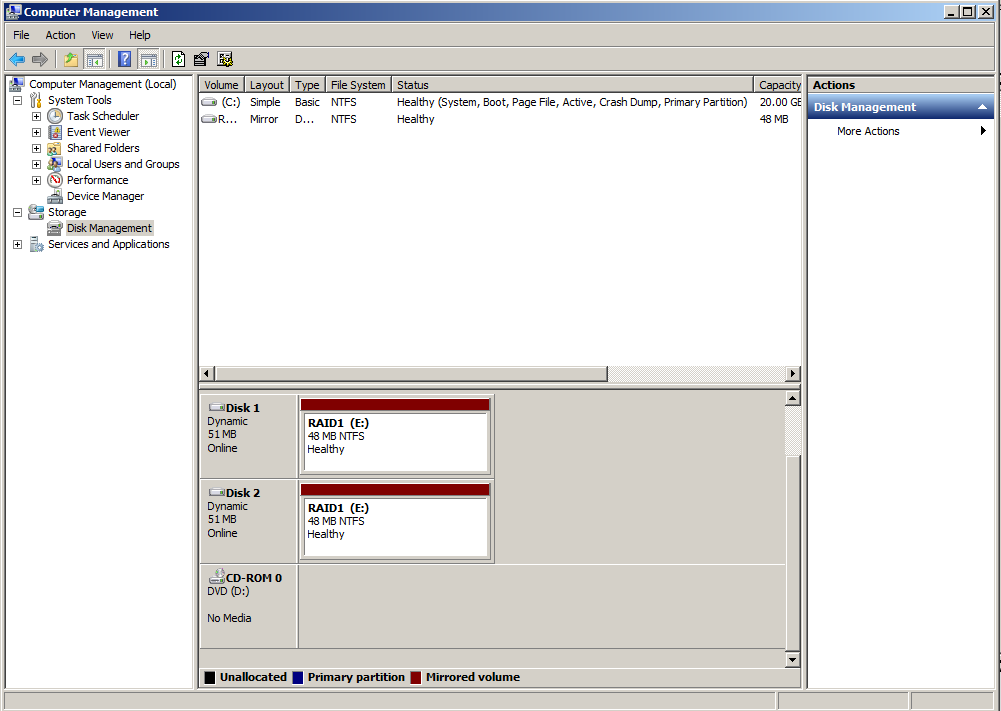
\includegraphics[width=0.8\textwidth]{images/15/5}
	\caption{RAID1 listo y funcionando}
	\label{fig:c1505}
\end{figure}
\clearpage
%----------------------------------------------------------------------------------------
%CUESTION 16
%----------------------------------------------------------------------------------------
\section{Con que opción establecemos una red local con la maquina anfitriona?¿Con que opción podemos compartir la conexión a Internet?}

a) Tenemos que seleccionar la Máquina Virtual sin arrancarla, editamos la configuración y poner la opción de tipo de Adaptador de Red (Netword Adapter) en modo “host-only”.\\\\
b) Con el modo NAT.\\


%----------------------------------------------------------------------------------------
% CUESTION 17
%----------------------------------------------------------------------------------------
\section{Como podemos ver que ambas maquinas están conectadas en la misma red local?(Pistas: ping, ifconfig, ifdown, ifup).Nota: al cambiar la configuración de VMSW hay que bajar y subir la interfaz de red para que la maquina virtual actualice sus parámetros.) Pruebe a ejecutar varias maquinas virtuales simultáneamente y compruebe que pueden “verse” entre ellas dentro de la misma red local.}

Podemos hacer un ping al broadcast de la subred que previamente conocemos con el comando ifconfig <adaptador>: ping –b <x.x.x.255>\\
	
	
	
	
	
%---------------------------------------------------------------------------------------
% CUESTION OPCIONAL 2 18
%----------------------------------------------------------------------------------------
\section{Cuestión opcional 2: ¿Que relación hay entre los atajos de teclado de emacs y los de la consola bash?.¿y entre los de vi y las paginas del manual?}

Los atajos de emacs son casi idénticos a los de bash ya que es desarrollado por GNU aunque se puede cambiar la configuración al estilo Vi/Vim escribiendo:  ‘set –o vi’.\\

Los atajos de las páginas del manual son idénticos a los del vi aunque internamente parece que no tienen que ver ya que las "man pages" no se basan en vi sino en "boost".





\clearpage
\bibliography{citas} %archivo citas.bib que contiene las entradas 
\bibliographystyle{unsrt} % hay varias formas de citar


\end{document}